\documentclass{article}
\usepackage{graphicx}
\usepackage[a4paper, left=2cm, right=2cm, top=2.5cm, bottom=2cm]{geometry}
\usepackage[small]{titlesec}
\usepackage{subcaption} 
\usepackage[italian]{babel}
\usepackage[hidelinks]{hyperref}
\usepackage{listings}
\usepackage{sectsty}
%\usepackage[light]{CormorantGaramond}
\usepackage{fancyhdr}
\usepackage{footnote}
\usepackage{tgadventor}
\usepackage{titling}
\usepackage{graphicx}
\usepackage{tcolorbox}
\usepackage{multirow}
\usepackage{booktabs}
\usepackage{makecell}
\usepackage{algpseudocode}
\usepackage{algorithm}
\usepackage{mathtools}
\usepackage{amssymb}


\setlength{\droptitle}{-5em}   % regola la posizione del titolo
\pretitle{\begin{center}\LARGE}   % imposta la dimensione della font del titolo
\posttitle{\end{center}}
%\lstset{language=C}
\renewcommand\bfdefault{bx}
\sectionfont{\fontsize{20.74}{15}\selectfont}
\subsectionfont{\fontsize{17.28}{15}\selectfont}
\subsubsectionfont{\fontsize{12}{15}\selectfont}
\title{}

\author{}
\date{\today}


\begin{document}
\pagestyle{fancy}
\fancyhf{}
%\rhead{\thepage}
%\lhead{\rightmark}
\rfoot{\thepage}
\lhead{\quad \leftmark}
\rhead{ \quad \rightmark}

\renewcommand{\headrulewidth}{0.2pt}



\begin{titlepage}
    \begin{figure}[t]
        \centering
        
\includegraphics[width=0.7\textwidth]{im/logo_sapienza_new.png}
        \label{fig:logo}
    \end{figure}    
    \null\vfill
    \begin{center}
      {\Huge Appunti di Basi Dati Modulo I} \\[2cm]
      {\Large Colacel Alexandru Andrei}
    \end{center}
    \vfill\null
    \renewcommand{\abstractname}{Disclaimer}

    
    
    \begin{abstract}  
    
    \hrulefill


    Le fonti sono le "Hand Notes" del prof. Perelli tradotte in italiano, appunti presi dalle slides della prof. De Marsico ed eventuali e-mail.\\
    \textbf{Nota: è vietata assolutamente la vendita di questo materiale in qualsiasi forma senza il mio consenso.} 
    \hrulefill
    \end{abstract}
  \end{titlepage}


\pagebreak
\tableofcontents

\pagebreak


\section{Lemma della Chiusura}
Sia $R$ uno schema e sia $F$ un insieme di dipendenze funzionali definite su $R$. Si ha che:\par 
\[X \rightarrow Y \in F^{A} \Longleftrightarrow Y \subseteq X^{+}\]

\subsection{Dimostrazione $\Rightarrow$}

Dato $X$ $\rightarrow$ $Y \in F^{A}$, per la regola della decomposizione, otteniamo:
\[X \rightarrow A \in F^{A}, \quad \forall A \in Y\]

e quindi, per definizione di $X^{+}$, otteniamo che: 

\[A \in X^{+}, \quad \forall A \in Y  \]

che significa: 

\[Y \subseteq X^{+}\]



\subsection{Dimostrazione $\Leftarrow$}
Dato: 
\[Y \subseteq X^{+}\]
si ottiene che: 

\[X \rightarrow A \in F^{A} \quad \forall A \in Y\]

che implica, per la regola dell'unione, che: 

\[X \rightarrow Y \in F^{A}\]


\pagebreak
\section{Teorema $F^{+}$ = $F^{A}$}

Dato uno schema $R$ e un insieme $F$ di dipendenze funzionali definite su $R$, si ha che:
\[ F^{+} = F^{A}\]


\subsection{Dimostrazione $F^{A} \subseteq F^{+}$}
Prendiamo $X \rightarrow Y \in F^{A}$, noi dobbiamo provare che $X \rightarrow Y \in F^{+}$ per induzione con $n$ numero di applicazioni degli assiomi di Armstrong.
\begin{itemize}
  \item \textbf{Caso base} (n = 0): se $X \rightarrow Y \in F^{A}$ senza aver applicato alcun assioma di Armstrong, allora l'unica possibilità è che:
  \[X \rightarrow Y \in F \subseteq F^{+}\]

  \item \textbf{Ipotesi induttiva forte:} ogni dipendenza funzionale in $F^{A}$ ottenuta da $F$
  applicando k $\leq$ n assiomi di Armstrong è anche in $F^{+}$:
  \begin{center}
    $X \rightarrow Y \in F^{A}$ tramite $k \leq n$ assiomi $\Rightarrow X \rightarrow Y \in F^{+}$
  \end{center}
  \item \textbf{Passo induttivo:} è necessario dimostrare che se $X \rightarrow Y \in F^{A}$ dopo aver applicato $n +1$ assiomi di Armstrong, allora $ X \rightarrow Y \in F^{+}$.\par
  È possibile ritrovarsi in uno dei seguenti tre casi:
  \begin{enumerate}
    \item Se l'$(n + 1)$-esimo assioma applicato è l'assioma di \textbf{riflessività}, allora l'unica possibilità è che:

    \[X \rightarrow Y \in F^{A} \Leftrightarrow Y \subseteq X \subseteq R\]

    Dunque, poiché, $Y \subseteq X \subseteq R$, per ogni istanza legale di $R$ si ha che:

    \[\forall t_1, t_2 \in r_{1}, t_1[X] = t_2[X] \Rightarrow t_1[Y] = t_2[Y]\]
    da cui ne segue automaticamente che $X \rightarrow Y \in F^{+}$
    \item Se l'$(n + 1)$-esimo assioma applicato è l'assioma di \textbf{aumento}, allora è obbligatoriamente necessario che:
    \begin{itemize}
      \item $\exists V, W \subseteq R \, | \, \exists V \rightarrow W \in F^{A}$, ottenuta applicando $j \leq n$ assiomi di Armstrong\\

      \item $\exists Z \subseteq R \, | \, X := VZ, \, Y := WZ$\\
    \end{itemize}
      Affinché si abbia che:

      \[Z \subseteq R, \, V \rightarrow W \Rightarrow VZ \rightarrow WZ = X \rightarrow Y \in F^{A}\]

      Siccome per ipotesi induttiva si ha $V \rightarrow W \in F^{A} \Rightarrow V \rightarrow W \in F^{+}$ e siccome $Z \subseteq Z \Rightarrow Z \rightarrow Z \in F^{+}$, si vede facilmente che: 
      \begin{figure}[hbt]
        \begin{center}
            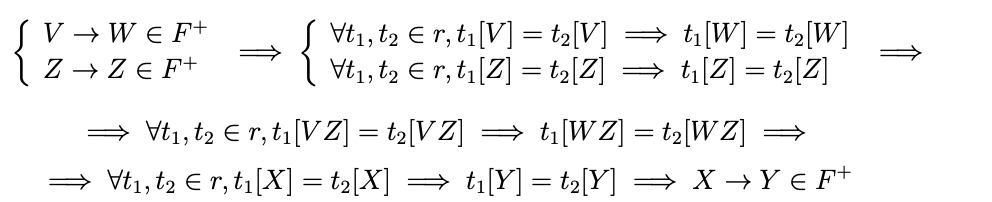
\includegraphics[width=0.8\textwidth,keepaspectratio]{{im/1}}
        \end{center}
        \end{figure}
        \pagebreak
      \item Se l'$(n + 1)$-esimo assioma applicato è l'assioma di \textbf{transitività}, allora è obbligatoriamente necessario che $\exists X \rightarrow Z, Z \rightarrow Y \in F^{A}$, ottenute con $k \leq n$ assiomi di Armstrong.

      %\[X \rightarrow Z \in F^{A} \lor Z \rightarrow Y \in F^{A} \Rightarrow X \rightarrow Y \in F^{A}\]

      Siccome per ipotesi induttiva $X \rightarrow Z \in F^{A} \Rightarrow X \rightarrow Z \in F^{+}$ e $Z \rightarrow Y \in F^{A} \Rightarrow Z \rightarrow Y \in F^{+}$, si vede facilmente che:
      \begin{figure}[hbt]
        \begin{center}
            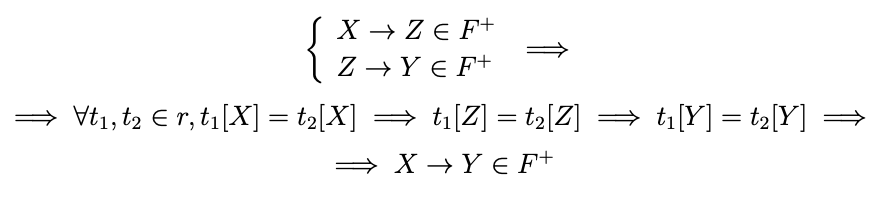
\includegraphics[width=0.7\textwidth,keepaspectratio]{{im/2}}
        \end{center}
        \end{figure}
  \end{enumerate}
\end{itemize}



\pagebreak
\subsection{Dimostrazione $F^{+} \subseteq F^{A}$}
\begin{figure}[hbt]
  \begin{center}
      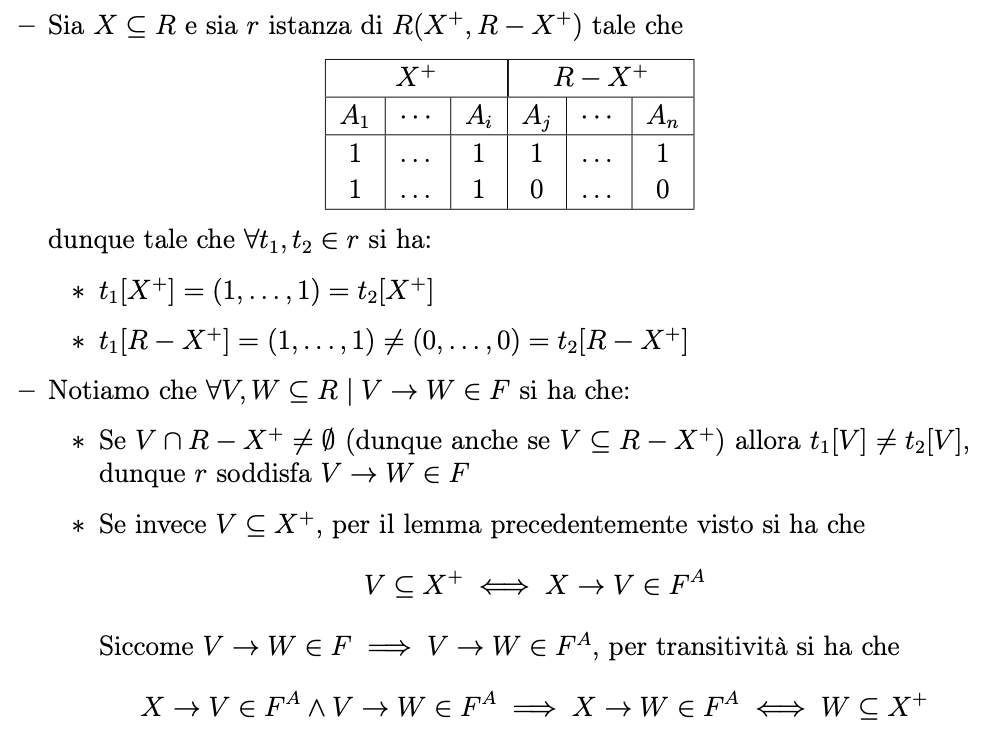
\includegraphics[width=0.75\textwidth,keepaspectratio]{{im/3}}
  \end{center}
  \end{figure}
  \begin{figure}[hbt]
    \begin{center}
        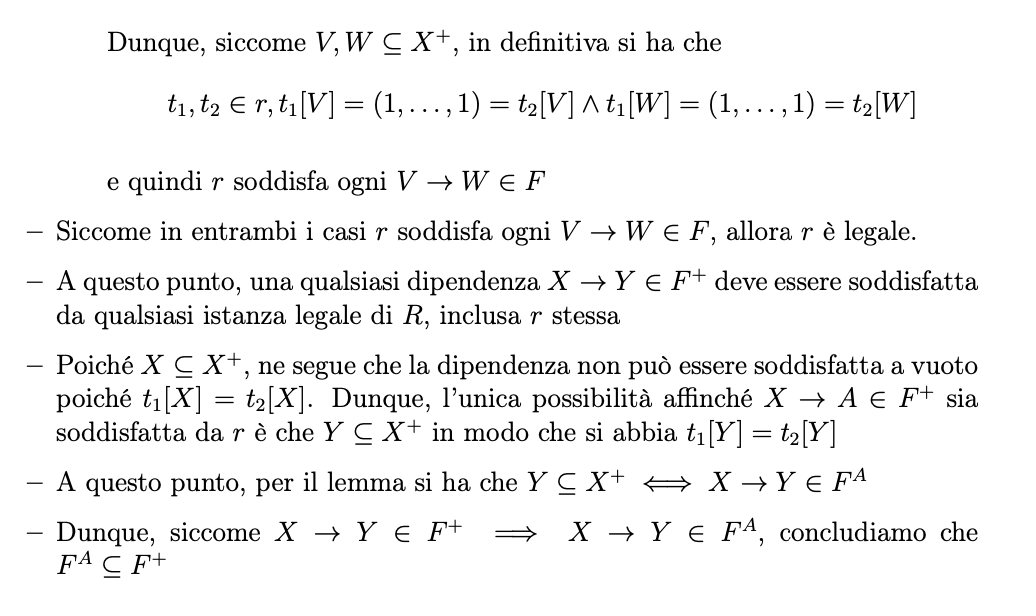
\includegraphics[width=0.8\textwidth,keepaspectratio]{{im/4}}
    \end{center}
    \end{figure}
    
    \begin{tcolorbox}[colback=white!20!white,colframe=green!70!black, title=Nota]
      Poiché $F^{+} = F^{A}$, per calcolare $F^{+}$ ci basta applicare gli assiomi di Armstrong sulle dipendenze in $F$ in modo da trovare $F^{A}$. \par Tuttavia, calcolare $F^{+} = F^{A}$ richiede tempo esponenziale, quindi $O(2^{nk})$: considerando anche solo l'assioma di riflessività, siccome ogni possibile sottoinsieme di $R$ genera una dipendenza e siccome i sottoinsiemi possibili di $R$ sono $2^{|R|}$, allora ne segue che $|F^{+}| >> 2^{|R|}$.
    \end{tcolorbox}
    \begin{figure}
      \begin{center}
          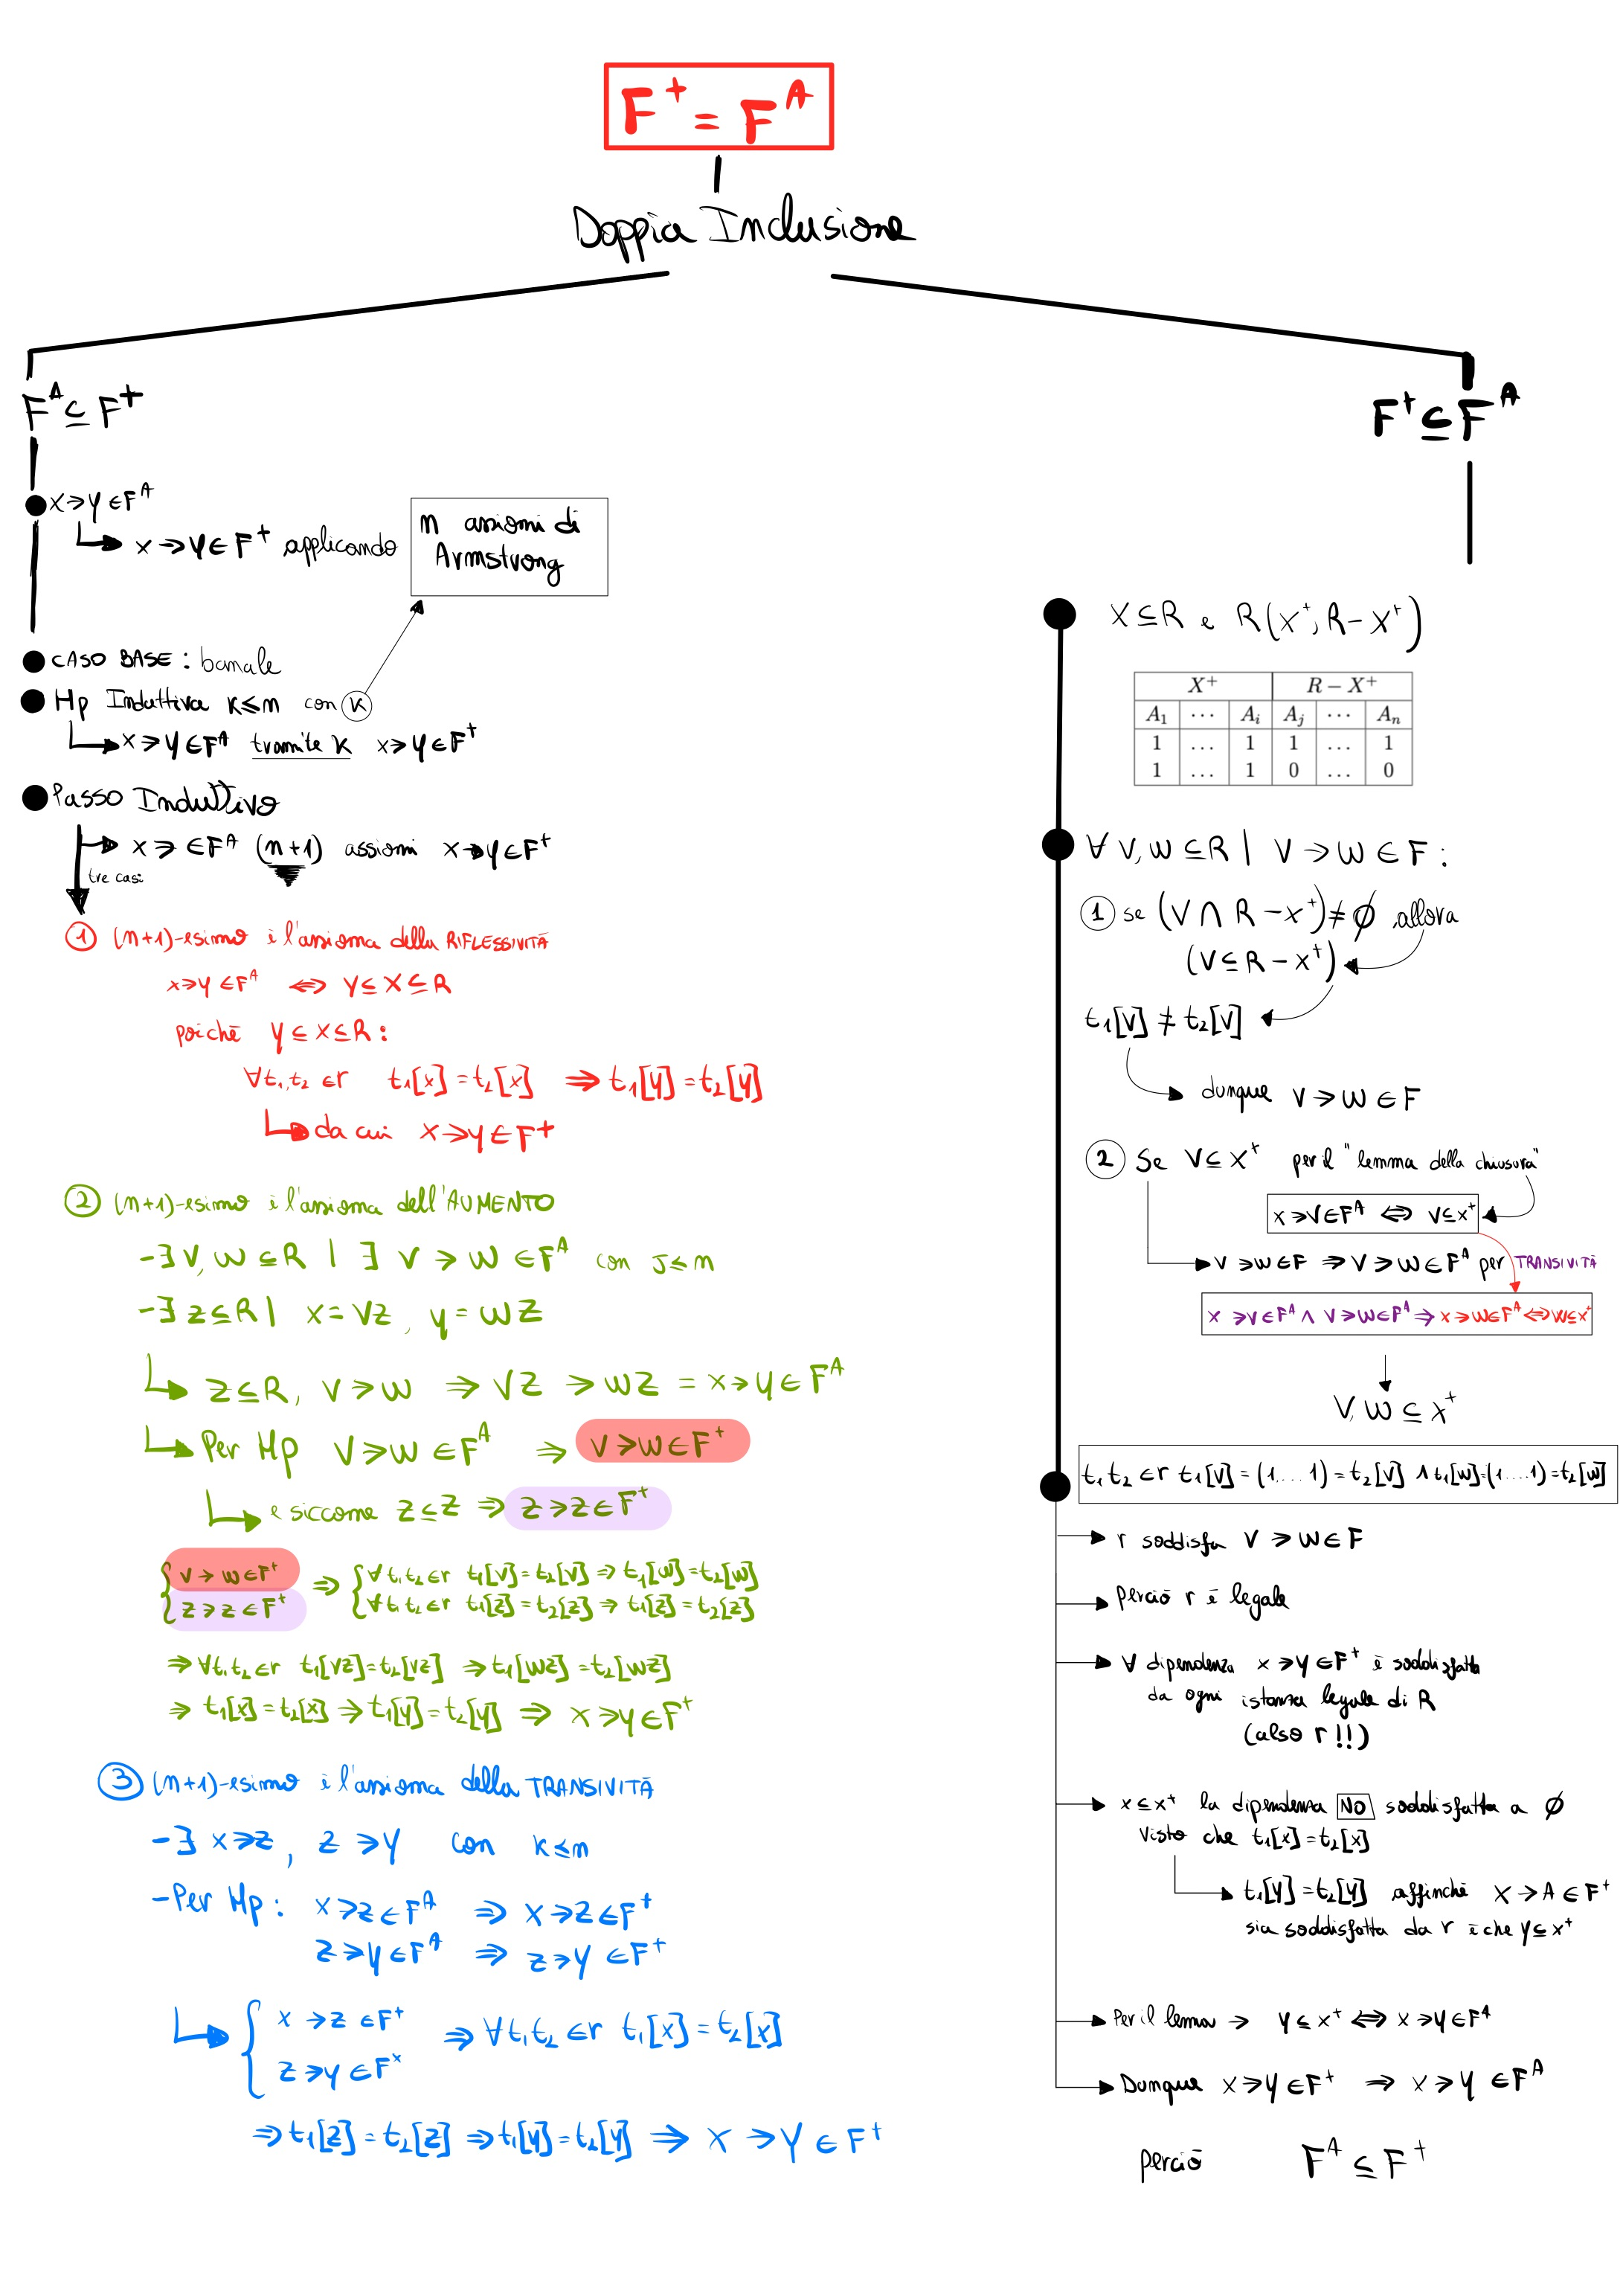
\includegraphics[width=1\textwidth,keepaspectratio]{{im/FA=F+}}
        \end{center}
      \end{figure}




\pagebreak
\section{Chiusura di X}
\subsection{Chiusura di un insieme di attributi}
Sia $R$ uno schema e sia $F$ un insieme di dipendenze funzionali definite su $R$.\\
 
Dato $X \subseteq R$, definiamo come chiusura di $X$ rispetto a $F$, indicata con $X_F^+$ (o solo $X^+$ se $F$ è l'unico insieme di dipendenze su $R$), il seguente insieme: 
\[X_F^+ = \{ A \in R \mid X \rightarrow A \in F^A \}\] dove $A \in R$ implica che $A$ sia un singolo attributo di $R$.\\
\texttt{Input}:
\begin{itemize}
  \item Relazione $R$
  \item Dipendenze Funzionali $F$
  \item Insieme $X \subseteq R$
\end{itemize}
\texttt{Output}: $X^{+}$

\begin{algorithm}
  \caption{Algoritmo per la chiusura di un insieme di attributi}  
    \begin{algorithmic}[1]
  \State $Z \gets X$
  \State $S \gets \{A \mid \exists Y \rightarrow V \in F, A \in V \land Y \subseteq Z\}$
  \While{$S \not\subseteq Z$}
    \State $Z \gets Z \cup S$
    \State $S \gets \{A \mid \exists Y \rightarrow V \in F, A \in V \land Y \subseteq Z\}$
  \EndWhile
  \State \textbf{return} $Z$
  \end{algorithmic}
\end{algorithm}
Tale algoritmo viene eseguito in tempo polinomiale, ossia $On^{k}$

\subsection{Teorema: L'algoritmo computa $X_{F}^{+}$}
Il teorema calcola correttamente la chiusura di un insieme di attributi X rispetto ad un insieme F di dipendenze funzionali.\\

\textbf{Dimostrazione Correttezza dell'algoritmo}:\\

Denotiamo:\par

\[Z_{0}, Z_{1}, \dots, Z_{i}, \dots \]
\[S_{0}, S_{1}, \dots, S_{i}, \dots\]\\

Indichiamo con $Z_{0}$ il valore iniziale di $Z (Z_{0} = X)$ e con $Z_{i}$ e $S_{i}$, $i \geq 1$ i valori di $Z$ ed $S$ dopo l'$i$-esima esecuzione del corpo del ciclo, infatti notiamo che $Z_{i} \subseteq Z_{i+1}$, per ogni $i$.\par
Sia $j$ tale che $S_{j} \subseteq Z_{j}$ (cioè,  $Z_{j}$ è l'output di $Z$ quando l'algoritmo termina); proveremo che:

\[A \in Z_{j} \Leftrightarrow A \in X^{+} \]
\begin{itemize}
  \item Dimostriamo per induzione su $i$ che $Z_{f} \subseteq X^{+}$
  \begin{itemize}
    \item \textbf{Caso base} i = 0:\par 
    Alla $0$-esima iterazione del while (ossia prima di esso) si ha $Z_{0} = X$ e $X \subseteq X^{+}$

    \item \textbf{Ipotesi induttiva}: Per ogni $i \in\mathbb{N}$ si ha che $Z_i \subseteq X^+$

    \item \textbf{Passo induttivo} ($i > 0$):
    Dato $A \in Z_{i+1} = Z_i \cup S_i$, si ha che $A \in Z_i \lor A \in S_i$. \par 
    Dunque, si possono verificare due casi:
    \begin{itemize}
      \item $\text{Se } A \in Z_i, \text{ allora per ipotesi } A \in Z_i \subseteq X^+.$
      \item $\text{Se } A \in S_i, \text{ allora } \exists Y \rightarrow V \in F \text{ tale che } A \in V \subseteq R, Y \subseteq Z_i.$\par
      Siccome per ipotesi  $Z_i \subseteq X^+ \text{ e } Y \subseteq Z_i$ allora: 
      \[Y \subseteq Z_i \subseteq X^+ \iff X \rightarrow Y \in F^A\] e 
      \[Y \rightarrow V \in F \implies Y \rightarrow V \in F^A\] 
      quindi per transitività si ha che:

      \[X \rightarrow Y, Y \rightarrow V \in F^A \implies X \rightarrow V \in F^A \iff V \subseteq X^+\]
      Dunque,si ha che $A \in V \subseteq X^+$
      \item $\text{Siccome in entrambi i casi } A \in Z_{i+1} \implies A \in X^+, \text{ allora concludiamo che } Z_{i+1} \subseteq X^+$.

    \end{itemize}
    
  \end{itemize}
  \pagebreak
  \item Dimostriamo ora che $X^{+} \subseteq Z_{i}$:\par
  \begin{itemize}
    \item Sia $X \subseteq R$ e sia $r$ istanza di $R(Z_{i}, R-Z_{i})$. 
    \begin{table}[ht]
      \centering
      \begin{tabular}{|c|c|c|c|c|c|}
      \hline
      \multicolumn{3}{|c|}{$Z_{i}$} & \multicolumn{3}{c|}{$R - Z_{i}$} \\
      \hline
      $A_1$ & $\dots$ & $A_{i}$ & $A_{j}$ & $\dots$  & $A_{n}$ \\
      \hline
      $1$ & $\dots$ & $1$ & $1$ & $\dots$  & $1$ \\
      \hline
      $1$ & $\dots$ & $1$ & $0$ & $\dots$  & $0$ \\
      \hline
      \end{tabular}
  \end{table}

Proviamo se legale:
  \begin{itemize}
    \item Prendiamo una dipendenza funzionale $V \rightarrow W \in F$
    \begin{itemize}
      \item Se $t_1[V] \neq t_2[V]$ allora $r$ soddisfa $V \rightarrow W$
      \item Se $t_1[V] = t_2[V]$ allora è verificato che $V \subseteq Z_i$. Otteniamo così che $W \subseteq S_i$, come ciascun attributo $B \in W$ è aggiunto a $S_i$ ciò significa che $V \rightarrow W \in F$
      \item Adesso se $Z_i$ terminale noi otteniamo $W \subseteq S_i \subseteq Z_i$ e quindi che $t_1[W] = t_2[W]$ perciò $r$ soddisfa $V \rightarrow W$
    \end{itemize} 
      \item Essendo $r$ un'istanza legale, noi abbiamo che $r$ soddisfa $X \rightarrow A$. Adesso visto che abbiamo $X \subseteq Z_0 \subseteq Z_i$ otteniamo che $t_1[X] = t_2[X]$ e quindi che $t_1[A] = t_2[A] \Rightarrow A \in Z_i$

  \end{itemize}
\end{itemize}
\end{itemize}
\begin{figure}
  \begin{center}
      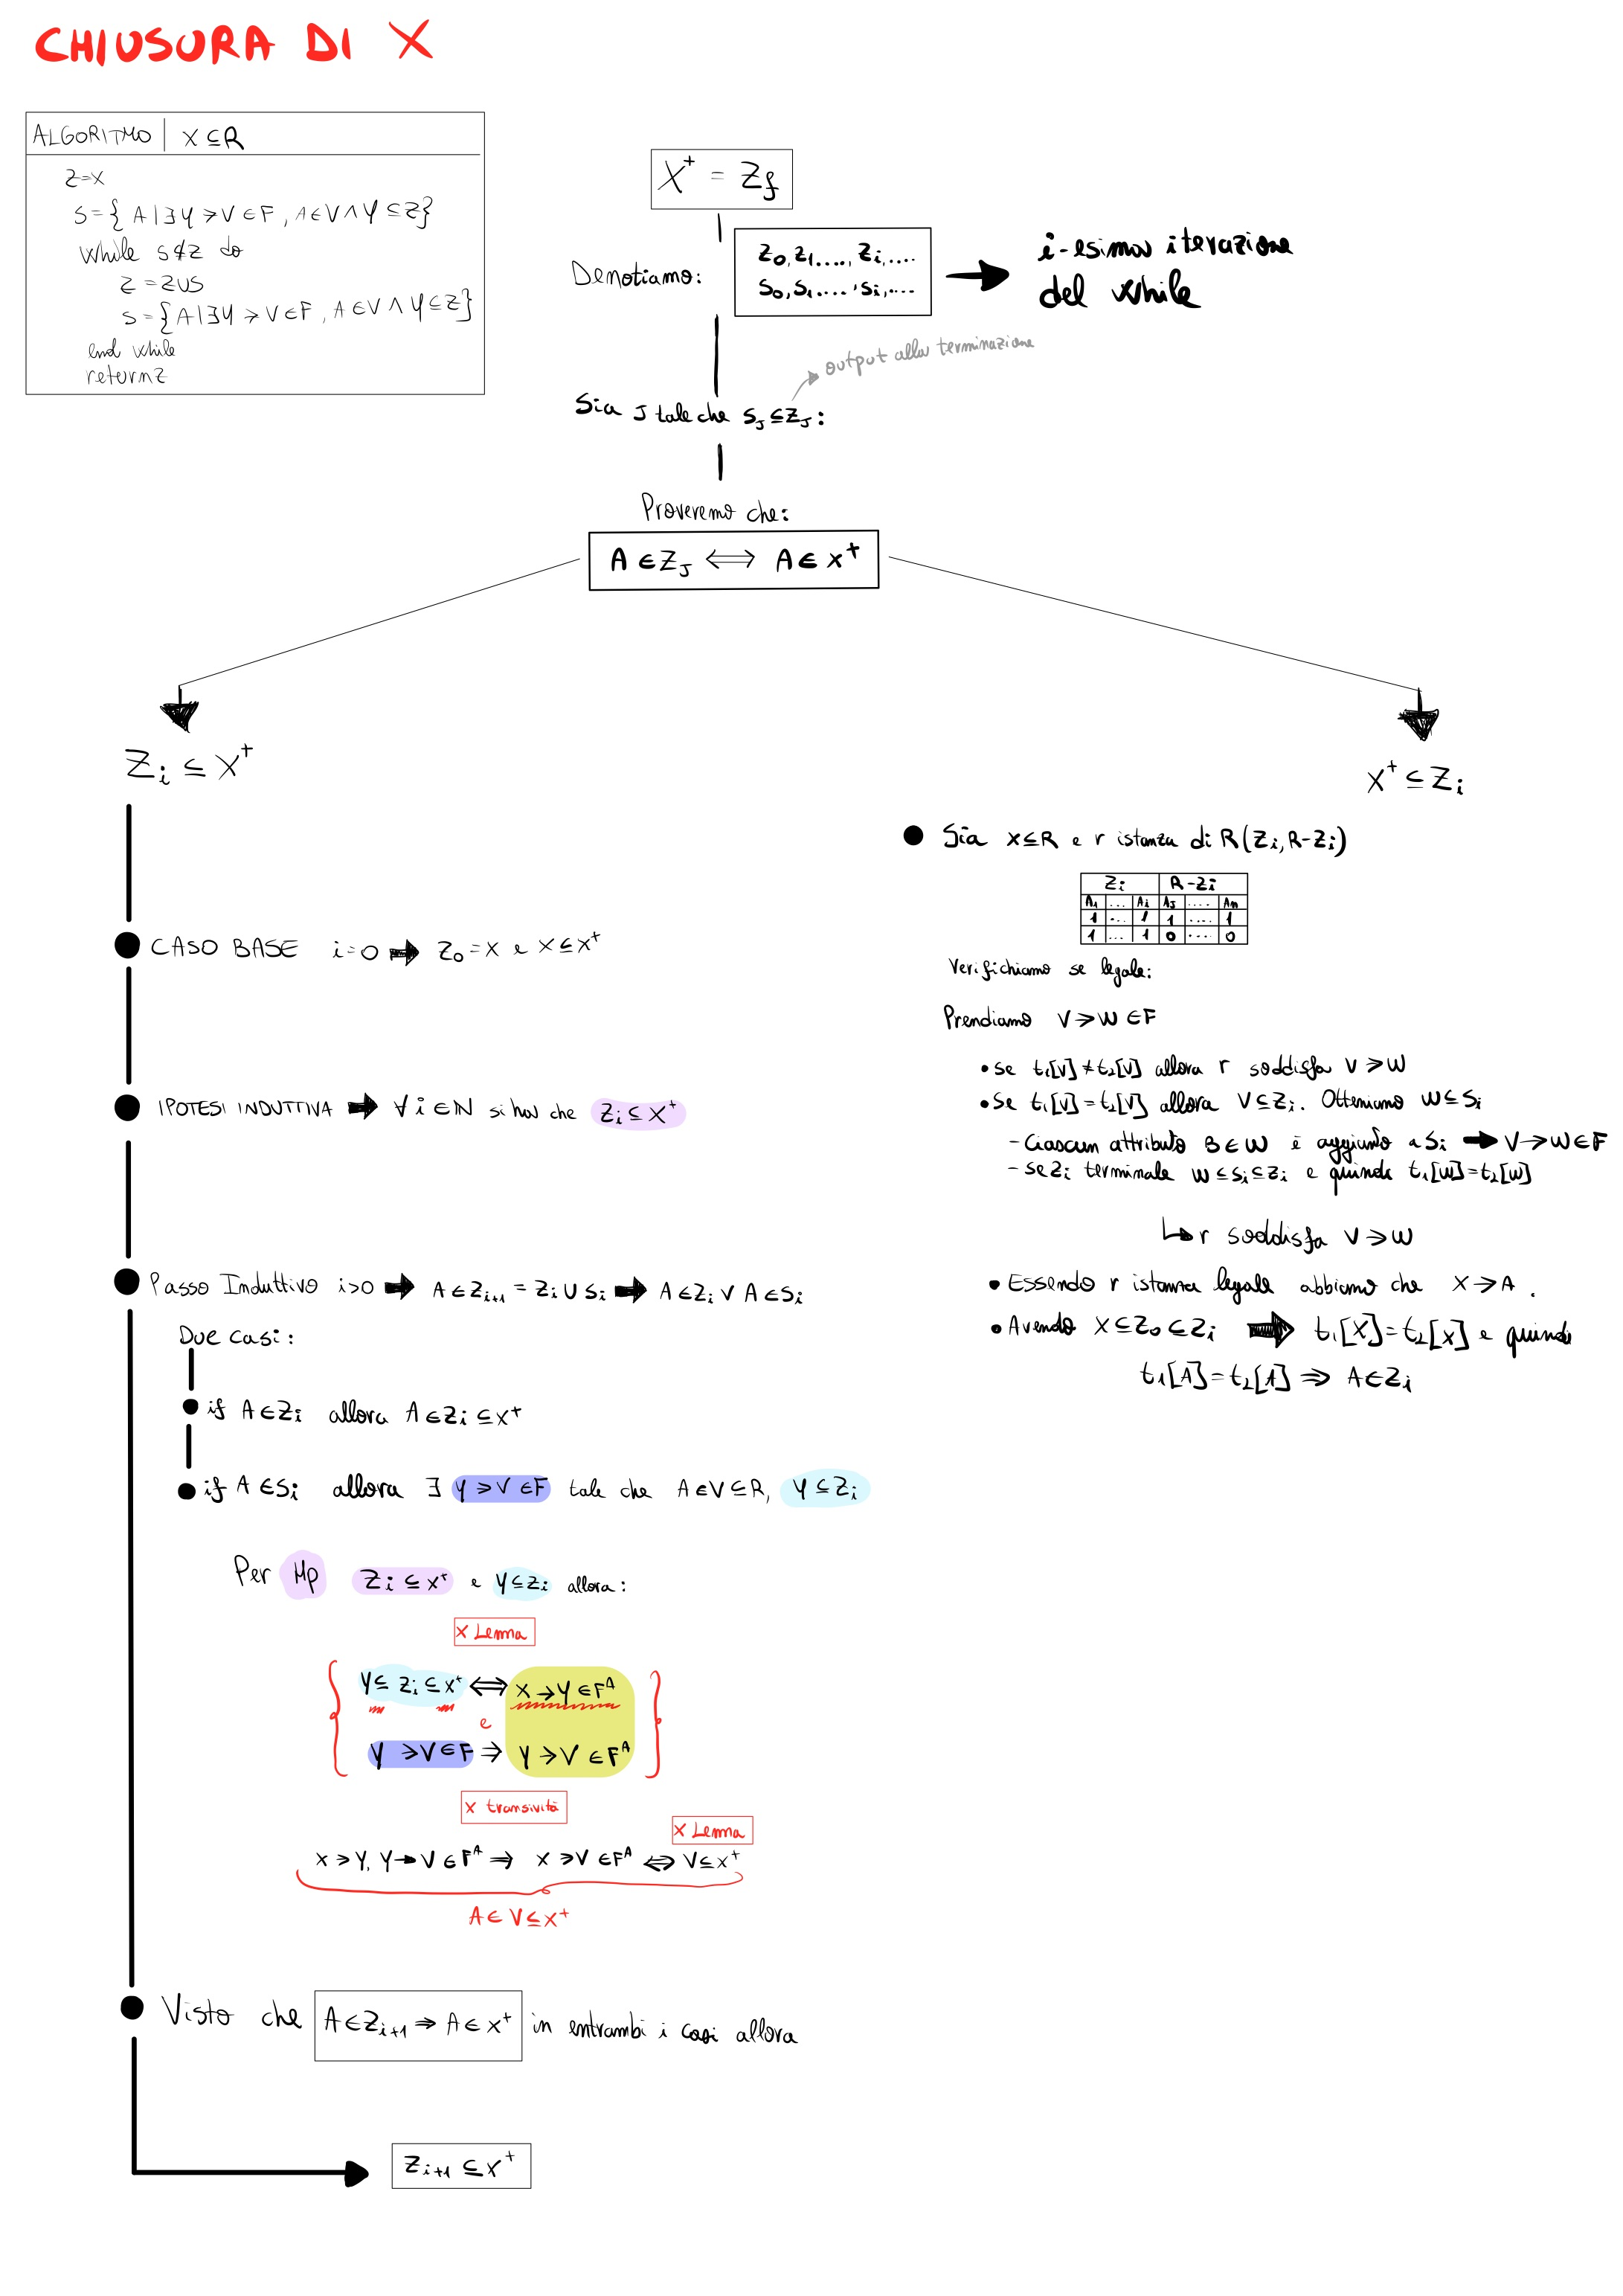
\includegraphics[width=1\textwidth,keepaspectratio]{{im/X}}
    \end{center}
  \end{figure}



\pagebreak
\section{Lemma: Inclusione delle chiusure}
Dato uno schema $R$ e due insiemi $F$ e $G$ di dipendenze funzionali su $R$, si ha che:\par 

\[F \subseteq G^+ \rightarrow F^+ \subseteq G^+\]

\subsection{Dimostrazione}
\begin{itemize}
  \item Denotiamo come $F \xrightarrow{\text{A}} F'$ la possibilità di ottenere $F'$ partendo da F applicando una determinata quantità di assiomi di Armstrong.
  \item  Ricordando che $F^A$ è l'insieme di tutte le dipendenze funzionali ottenibile applicando assiomi di Armstrong su $F$.
  \item Otteniamo che $F \xrightarrow{\text{A}} F' \Leftrightarrow F' \subseteq F^+$ e in particolare $F \rightarrow F^+$
  \item Adesso abbiamo ottenuto che $F \subseteq G^+ \Leftrightarrow G \xrightarrow{\text{A}} F \xrightarrow{\text{A}} F^+$ 
  \item Quindi $G \xrightarrow{\text{A}} F^+$ il quale implica che \textbf{$F^+ \subseteq G^+$}

\end{itemize}







\pagebreak
\section{Chiusura di $X$ in $G$}
Dato uno schema R con decomposizione $\rho$ = $R_1,...,R_k$, dato un insieme $F$ di dipendenze funzionali su $R$ e posto:
\[ G := \bigcup_{i=0}^{k} \pi_{R_i}(F) \]\par
preso $X \subseteq R$, il seguente algoritmo calcola $X_G^+$ tramite $F$:
\begin{algorithm}
  \caption{Calcolo di $X_G^+$ tramite $F$}
  \begin{algorithmic}[1]
      \Procedure{Calculate$X_G^+$}{$R$: schema, $F$: set of dependencies, $X$: set of attributes}
          \State $Z \gets X$
          \State $S \gets \emptyset$
          \For{$i \gets 1$ to $k$}
              \State $S \gets S \cup ((Z \cap R_i)^+_F \cap R_i)$
          \EndFor
          \While{$S \not\subseteq Z$}
              \State $Z \gets Z \cup S$
              \For{$i \gets 1$ to $k$}
                  \State $S \gets S \cup ((Z \cap R_i)^+_F \cap R_i)$
              \EndFor
          \EndWhile
          \State $X_G^+ \gets Z$
          \State \textbf{return} $X_G^+$
      \EndProcedure
  \end{algorithmic}
\end{algorithm}

\subsection{Dimostrazione}
\begin{itemize}
  \item Siano $Z_0,Z_1, \dots,Z_i, \dots$ e $S_0,S_1,\dots ,S_i,\dots$ gli insiemi calcolati ad ogni iterazione del ciclo while dell'algoritmo
  \item Osserviamo che $Z_i \subseteq Z_{i+1}$ per ogni $i \in \mathbb{N}$, dunque $Z_0, Z_1, \ldots, Z_i, \ldots$ è una sequenza monotona limitata da $R$, implicando che esiste un $f \in \mathbb{N}$ tale che $Z_f = Z_{f+1}$
  \item Siccome ciò può accadere solo se $S_f \subseteq Z_f$, ossia quando l'algoritmo termina, si ha che $Z_f$ è l'output dell'algoritmo
  \item Dimostriamo per induzione che $Z_f \subseteq X_G^+$:
  \begin{itemize}
    \item \textbf{Caso base ($i = 0$):} \\
    Alla 0-esima iterazione del \texttt{while}, prima di esso, si ha $Z_0 = X \subseteq X_G^+$.
    
    \item \textbf{Ipotesi induttiva:} \\
    Per ogni $i \in \mathbb{N}$ si ha che $Z_i \subseteq X_G^+$.
    
    \item \textbf{Passo induttivo ($i > 0$):} \\
    Dato $A \in Z_{i+1} = Z_i \cup S_i$, abbiamo che $A \in Z_i$ oppure $A \in S_i$. Quindi possiamo considerare due casi:
    
    \begin{itemize}
      \item Se $A \in Z_i$, allora per ipotesi induttiva abbiamo che $A \in Z_i \subseteq X_G^+$.
      \item Se $A \in S_i$, allora per la definizione stessa di $S_i$, $\exists$ $j \leq k$ tale che $A \in ((Z_i \cap R_j)^+_F \cap R_j)$.\\
      
      A questo punto, abbiamo che:\\

      $A \in ((Z_i \cap R_j)^+_F \cap R_j)$ $\Leftrightarrow$ $A \in (Z_i \cap R_j)^+_F$ $\land$ $A \in R_j$ \\ 

      da cui otteniamo che:\\ 
      
      $A \in (Z_i \cap R_j)^+_F$ $\Leftrightarrow$ $(Z_i \cap R_j) \rightarrow A \in F^A = F^+$. \\
      
      Dunque, siccome $(Z_i \cap R_j) \subseteq R_j$ e $A \in R_j$, allora si ha che:\\

        $(Z_i \cap R_j) \rightarrow A \in \pi_{R_j}(F) = \{X \rightarrow Y \in F^+ \,|\, XY \in R_j\}$
      
      
    Dai quali deduciamo che:\\

    $(Z_i \cap R_j) \rightarrow A \in \pi_{R_j}(F) \subseteq G \subseteq G^+ = G^A$.\\

    Inoltre, siccome $(Z_i \cap R_j) \subseteq Z_i$ e, per ipotesi induttiva, $Z_i \subseteq X_G^+$, otteniamo che:\\ 
    
    $(Z_i \cap R_j) \subseteq Zi \subseteq X_G^+$ \\
    
    implicando quindi che $X \rightarrow (Z_i \cap R_j) \in G^A$.

    Infine, per transitività otteniamo che:
    \[ X \rightarrow (Z_i \cap R_j), \, (Z_i \cap R_j) \rightarrow A \in G^A \Rightarrow X \rightarrow A \in G^A \Rightarrow A \in X_G^+ \]
    \end{itemize}  
    \item Dunque, siccome in entrambi i casi si ha $A \in Z_f \Rightarrow A \in X_G^+$, possiamo concludere che $Z_f \subseteq X_G^+$.

  \end{itemize}
  \item Dimostriamo per induzione che $X_G^+ \subseteq Z_f$\footnote{Dalle slides del Prof "Hand Notes" che \textbf{NON} sono oggetto di orale}:
  \begin{itemize}
    \item Osserviamo che $X \subseteq Y \Rightarrow X_F^+ \subseteq Y^+_F$
    \item Adesso sippiamo che $X = Z_0 \subseteq Z_f$, noi otteniamo che $X_G^+ \subseteq (Z_f)^+_G$. Noi possiamo dimostrare che $Z_f = (Z_f)^+_G$ che prova questo stato. Ovviamente $Z_f \subseteq (Z_f)^+_G$
    \item Dobbiamo ora dimostrare l'Inclusione. Consideriamo $S_1 = { A | Y \rightarrow V \in G, Y \subseteq Z_f, A \in V }$ e otteniamo per l'esecuizione del primo passo della chiususa dell'algoritmo di $Z_f$ su $G$. Noi abbiamo dimostrare che $S_1 \subseteq Z_f$. Poniamo $A \in S_1$. Questo significa che esiste $Y \rightarrow V \in G$ tale che $Y \subseteq Z_f$ e $A \in V$.
    \item Adesso per definizione di F, esiste un indice $j$ che $Y, V \subseteq R_j$ che significa $Y \subseteq Z_f \cap R_j$ e $A \in R_j$ e implica che $A \in (Z_j \cap R_j)^+_F \cap R_j$.
    \item Detto questo $A \in S_f \subseteq Z_f$ 
  \end{itemize}
\end{itemize}

Abbiamo dimostrato che \textbf{$Z_f = X_G^+$}
\pagebreak


\section{Join senza perdita}
Una decomposizione ha un join senza perdita se per ogni istanza legale \textit{r} di $R$ si ha che \textit{r} è ottenibile facendo il join naturale tra le proiezioni delle decomposizioni in $\rho$ di \textit{r}.
\\

\textbf{Teorema}
Sia $R$ uno schema con decomposizione $\rho = R_1, \ldots, R_k$ e sia $F$ un insieme di dipendenze funzionali su $R$. La decomposizione $\rho$ presenta un join senza perdita se per ogni istanza legale $r$ di $R$ si ha che:
\[ r = m_{\rho}(r) := \pi_{R_1}(r) \bowtie \ldots \bowtie \pi_{R_k}(r) \]

Sia $R$ uno schema con decomposizione $\rho = R_1, \ldots, R_k$ e sia $F$ un insieme di dipendenze funzionali su $R$. Posto $m_{\rho}(r) := \pi_{R_1}(r) \bowtie \ldots \bowtie \pi_{R_k}(r)$, per ogni istanza legale $r$ di $R$ si ha che:

\begin{enumerate}
  \item $r \subseteq m_{\rho}(r)$
  \item $\pi_{R_i}(m_{\rho}(r)) = \pi_{R_i}(r)$, per ogni $R_i \in \rho$
  \item $m_{\rho}(m_{\rho}(r)) = m_{\rho}(r)$
\end{enumerate}
\subsection{Dimostrazione $r \subseteq m_{\rho}(r)$}
Data una qualsiasi tupla $t \in r$, si ha che:
\[ t \in r \Rightarrow t \in \{t[R_1]\} \bowtie \ldots \bowtie \{t[R_k]\} \subseteq \pi_{R_1}(r) \bowtie \ldots \bowtie \pi_{R_k}(r) = m_{\rho}(r) \]
dunque $r \subseteq m_{\rho}(r)$.
\subsection{Dimostrazione  $\pi_{R_i}(m_{\rho}(r)) = \pi_{R_i}(r) \forall R_i \in \rho$}

Poiché $r \subseteq m_{\rho}(r)$, allora effettuando una proiezione con $R_i \in \rho$ su entrambe, ne segue che $\pi_{R_i}(r) \subseteq \pi_{R_i}(m_{\rho}(r))$.

Inoltre, per definizione di proiezione, si ha che:
\[ t \in \pi_{R_i}(m_{\rho}(r)) \Rightarrow \exists t' \in m_{\rho}(r) \text{ tale che } t_{R_i} = t^{'}[R_i] \]

Infine, per definizione stessa di $m_{\rho}(r)$, si ha che:
\[ t' \in m_{\rho}(r) \Rightarrow \exists t_1, \ldots, t_k \in r \text{ tale che } \forall R_j \in \rho, t_j[R_j] = t^{'}[R_j] \]

In particolare, quindi, otteniamo che:
\[ t_{R_i} \in \pi_{R_1}(m_{\rho}(r)) \Rightarrow t_{R_i} = t^{'}[R_i] = t_i[R_i] \in \pi_{R_i}(r) \Rightarrow \pi_{R_1}(m_{\rho}(r)) \subseteq \pi_{R_i}(r) \]

\subsection{Dimostrazione $m_{\rho}(m_{\rho}(r)) = m_{\rho}(r)$}
Siccome $\pi_{R_i}(r) = \pi_{R_1}(m_{\rho}(r))$, allora si ha che:
\[ m_{\rho}(m_{\rho}(r)) = \pi_{R_1}(m_{\rho}(r)) \bowtie \ldots \bowtie \pi_{R_k}(m_{\rho}(r)) = \pi_{R_1}(r) \bowtie \ldots \bowtie \pi_{R_k}(r) = m_{\rho}(r) \]

\pagebreak

\subsection{Algoritmo controllo presenza join senza perdita}
Dato uno schema $R = A_1, \ldots, A_n$ con decomposizione $\rho = R_1, \ldots, R_k$ e un insieme $F$ di dipendenze funzionali su $R$, presa l'istanza legale $r$ di $R$ dove per ogni $i \in [1, k]$ e per ogni $j \in [1, n]$ si ha:


Un sistema di equazioni con l'ambiente \texttt{cases}:
\[r_{i, j}
\begin{cases}
    "a" \quad se A_j \in R \\
    "b_i" \quad se A_j \notin R
\end{cases}
\]
il seguente algoritmo determina se $\rho$ presenta un join senza perdita.
\begin{algorithm}
  \caption{Verifica se $\rho$ ha un join senza perdita}
  \begin{algorithmic}[1]
      \Function{HasLosslessJoin}{$R, F, \rho$}
          \State $unchanged \gets \text{False}$
          \While{not $unchanged$}
              \State $unchanged \gets \text{True}$
              \For{$X \rightarrow Y \in F$}
                  \For{t1 in r}
                      \For{t2 in r}
                          \If{$t1[X] = t2[X]$ \textbf{and} $t1[Y] \neq t2[Y]$}
                              \State $unchanged \gets \text{False}$
                              \For{$A_j \in Y$}
                                  \If{$t1[A_j] = "a"$}
                                      \State $t2[A_j] \gets t1[A_j]$
                                  \Else
                                      \State $t1[A_j] \gets t2[A_j]$
                                  \EndIf
                              \EndFor
                          \EndIf
                      \EndFor
                  \EndFor
              \EndFor
          \EndWhile
          \For{$t \in r$}
              \If{$t = ("a", \ldots, "a")$}
                  \State \Return \text{True}
              \EndIf
          \EndFor
          \State \Return \text{False}
      \EndFunction
  \end{algorithmic}
\end{algorithm}
\pagebreak
\subsubsection{Commenti sull'algoritmo}
\begin{itemize}
    \item L'algoritmo modifica l'istanza di partenza $r$ in modo che tutte le dipendenze di $F$ vengano soddisfatte
    \item Ogni volta che l'algoritmo trova due tuple aventi lo stesso valore nel determinante ma valori differenti, quest'ultimo viene modificato in modo che essi siano uguali.
    \item Nel fare ciò, il simbolo "a" viene considerato prioritario, ovvero "a" non può mai diventare "b", mentre "b" può diventare "a".
    \item Se due tuple hanno lo stesso valore nel determinante ma valori differenti nel determinato, e solo una delle due tuple ha un valore "a" nel determinato, il valore "b" dell'altra tupla viene cambiato in "a".
    \item Se due tuple hanno lo stesso valore nel determinante ma valori differenti nel determinato, ma nessuna delle due tuple ha un valore "a" nel determinato, il valore "b" di una delle due tuple viene cambiato in modo che esse abbiano lo stesso valore "b".
    \item Due valori vengono considerati uguali se sono entrambi "a" (indipendentemente dal pedice che hanno) o se entrambi hanno una "b" con lo stesso identico pedice.
    \item L'algoritmo termina quando tutte le coppie di tuple soddisfano le dipendenze di $F$.
    \item Infine, $r$ diventa un'istanza legale di $R$.
    \item Una volta terminato l'algoritmo, se esiste almeno una tupla avente tutti valori "a" al suo interno, allora $\rho$ presenta un join senza perdita, altrimenti no.
\end{itemize}



\begin{figure}
  \begin{center}
      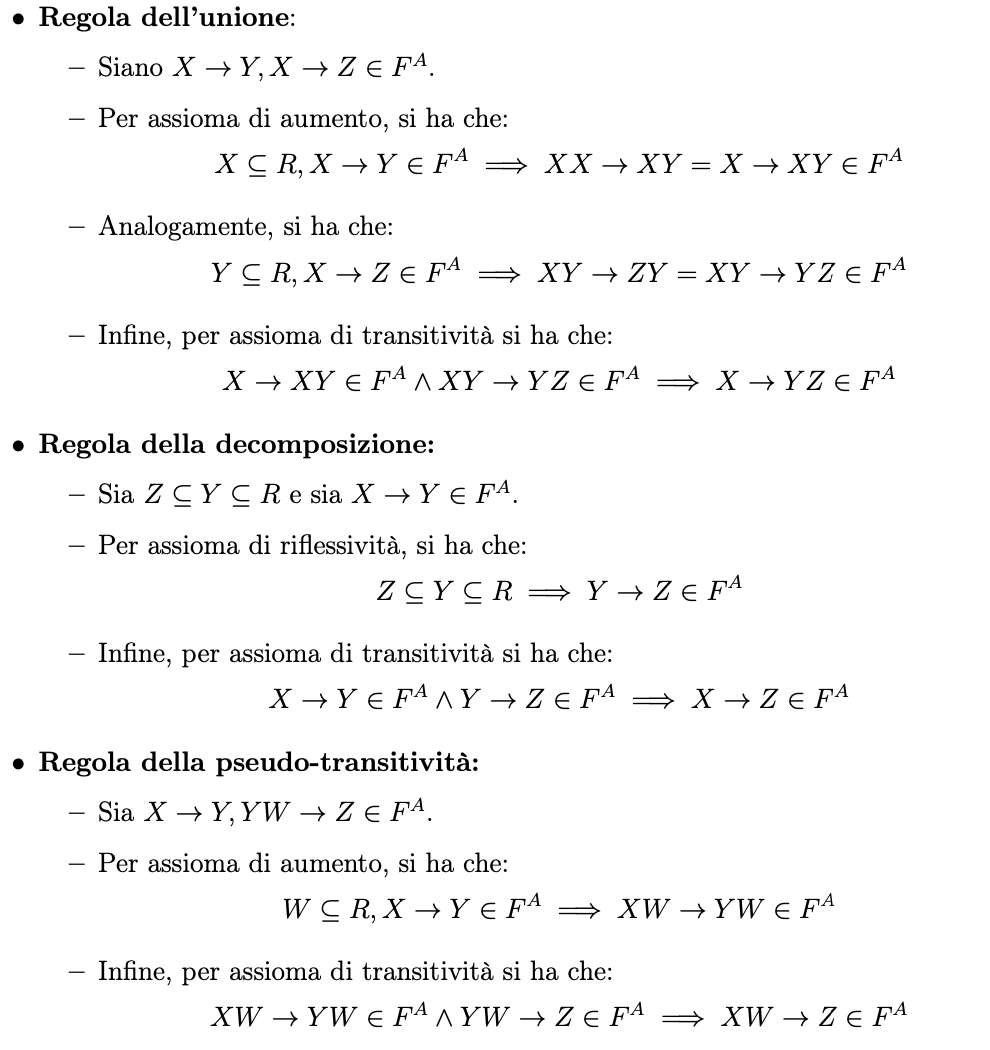
\includegraphics[width=1\textwidth,keepaspectratio]{{im/U}}
    \end{center}
  \end{figure}



\section{Assiomi di Armstrong}
Denotiamo con $F^A$ l'insieme di dipendenze funzionali definito nel modo seguente:

\begin{itemize}
  \item Se $f\in F$, allora $f\in F^A$.
  \item Se $Y\subseteq X\subseteq R$, allora $X\to Y\in F^A$ (\textbf{assioma della riflessività}).
  \item Se $X\to Y\in F^A$ e $Z\subseteq R$, allora $XZ\to YZ\in F^A$ (\textbf{assioma dell'aumento}).
  \item Se $X\to Y\in F^A$ e $Y\to Z\in F^A$, allora $X\to Z\in F^A$ (\textbf{assioma della transitività}).
\end{itemize}

Introduciamo altre tre regole conseguenza degli assiomi che consentono di derivare da dipendenze \par funzionali $F^A$ altre dipendenze funzionali in $F^A$:

\begin{itemize}
  \item Se $X\to Y\in F^A$ e $X\to Z\in F^A$, allora $X \to YZ\in F^A$ (\textbf{regola dell'unione}).
  \item Se $X\to Y\in F^A$ e $Z\subseteq Y$, allora $X \to Z\in F^A$ (\textbf{regola della decomposizione}).
  \item Se $X\to Y\in F^A$ e $WY\to Z\in F^A$, allora $WX\to Z\in F^A$ (\textbf{regola della pseudotransitività}).
\end{itemize}





\pagebreak


\section{Definizioni utili}
\subsubsection{Cos'è una dipendenza funzionale?}
Una dipendenza funzionale su una relazione $R$ è una coppia ordinata di sottoinsiemi di $R$ e viene denotata con $X \rightarrow Y$.\\

\subsubsection{Cos'è la chiusura di un insieme di dipendenze funzionali?}
La chiusura di un insieme di dipendenze funzionali è l'insieme di dipendenze funzionali soddisfatte da ogni istanza legale di $R$, essa viene denotata con $F^+$.\\

\subsubsection{Quali sono le caratteristiche di una chiave per una relazione?}
Un sottoinsieme $K$ di $R$ è chiave per $R$ se è un insieme minimale che determina $R$. Ovvero se $K \rightarrow R$ appartiene a $F^+$ e non esiste un $K'$ sottoinsieme di $K$ tale che $K' \rightarrow R$ appartiene a $F^+$.\\

\subsubsection{Cos'è un attributo primo?}
Un attributo si dice primo se appartiene a una chiave di $R$.\\

\subsubsection{Cos'è un superchiave?}
Un sottoinsieme $X$ di $R$ è una superchiave se contiene una chiave di $R$.\\

Sia $R$ uno schema e sia $F$ un insieme di dipendenze funzionali definite su $R$. Definiamo il sottoinsieme di attributi $K \subseteq R$ come superchiave di $R$ se:
\begin{itemize}
    \item $K \rightarrow R \in F^+$
    \item $\exists K' \subseteq K \,|\, K' \rightarrow R \in F^+ \land \nexists K'' \subset K' \,|\, K'' \rightarrow R \in F^+$ (ossia contiene una chiave)
\end{itemize}

\subsubsection{Definizione di decomposizione}
Sia $R$ uno schema. Definiamo come decomposizione di $R$ l'insieme di sottoschemi
$\rho$ = $R_1, \cdots,R_k$ che ricoprono $R$, ossia tali che:
\[ R := \bigcup_{i=0}^{k} R_i \]
In altre parole, $R_1, \cdots , R_k$ sono un insieme di schemi tramite cui è possibile ricostruire $R$ effettuando un join naturale tra essi.

\subsubsection{Decomposizioni che preservano i dati}


\subsubsection{Collegamento tra $F^+$ e $X_F^+$}

\subsubsection{Chiave Minimale (chiave primaria)}
Una chiave minimale, anche nota come chiave primaria, è un insieme di attributi (colonne) all'interno di una tabella (relazione) che può essere utilizzato per identificare univocamente ogni riga all'interno di quella tabella.
\begin{itemize}
  \item \textbf{Unicità}: Ogni valore nell'insieme di attributi deve essere unico all'interno della tabella. Non possono esistere due righe con lo stesso valore per l'insieme di attributi che costituisce la chiave minimale.
  \item \textbf{Irreducibilità}: Nessun sottoinsieme dell'insieme di attributi può conservare la proprietà di unicità. Questo significa che se si rimuove un qualsiasi attributo dall'insieme di attributi della chiave, la capacità di identificare univocamente le righe viene persa.
\end{itemize}

\subsubsection{Cos'è una copertura minimale di un insieme di dipendenze funzionali?}
Una copertura minimale di un insieme di dipendenze F è un insieme di dipendenze nel quale:
\begin{itemize}
  \item Ogni dipendenza funzionale ha la parte sinistra che è un singleton
  \item Ogni dipendenza funzionale ha la parte sinistra non ridondante
  \item Non sono presenti dipendenze funzionali ridondanti
\end{itemize}



\subsubsection{Cosa sono le dipendenze parziali e le dipendenze transitive?}
Una dipendenza $X \rightarrow A$ in $F^+$ si dice parziale se $A$ non è primo e $X$ è contenuto propriamente in una chiave. Una dipendenza $X \rightarrow A$ in $F^+$ si dice transitiva se $A$ non è primo ed $X$ non è contenuto in nessuna chiave $K$ in $R$ e $K - X \neq \emptyset$.\\

\subsubsection{Terza Forma Normale (3NF)}
Sia R uno schema e sia F un insieme di dipendenze funzionali definite su R. Lo schema R viene detto in terza forma normale (3NF) se:

\[\forall X \rightarrow A \in F^+, \, A \in R - X, \, \exists K \subseteq R \text{chiave} \,|\, K \subseteq X \vee A \in K\]

In altre parole, uno schema viene detto in terza forma normale se per ogni dipendenza funzionale non banale $X \rightarrow A \in F^+$, il determinante X è superchiave o il determinato A è primo.
Se uno schema è in 3NF, la quantità di anomalie e di ridondanze dei dati è estremamente ridotta.

\subsubsection{Quando è che una relazione è in 3NF? (Dimostra l'equivalenza tra le due affermazioni)}
\begin{itemize}
  \item Una relazione $R$ è in 3NF se per ogni dipendenza funzionale $X \rightarrow A$ in $F^+$ si ha che $A$ è primo oppure $X$ è una superchiave. \item Una relazione $R$ è in 3NF se in $F^+$ non ci sono né dipendenze \textbf{transitive} né dipendenze \textbf{parziali}.\\
\end{itemize}

\subsubsection{$F^A$}
Definiamo come $F^A$ l'insieme di tutte le dipendenze funzionali ottenibili assioma di aumento partendo da $F$ applicando i seguenti assiomi di Armstrong.

\subsubsection{Decomposizione che preserva F e Spiegazione}
Una decomposizione $\rho$ preserva un insieme di dipendenze funzionali $F$ se e solo se $F \equiv G$ dove (definizione di G):
\[ G := \bigcup_{i=1}^{k} \{X \rightarrow Y \mid X \rightarrow Y \in F^+ \land XY \subseteq R_i \} \]

\textbf{Spiegazione}: Proiettare ogni dipendenza funzionale in $F$ sul sottoschema $R_i$ vuol dire prendere in considerazione tutte e sole le dipendenze derivabili da $F$ (tramite assiomi di Armstrong, quindi $F^+$) che hanno tutti gli attributi in $R_i$


\subsection{Organizzazione con file Heap}
\begin{itemize}
  \item È il modello di organizzazione dei file primaria più basilare
  \item I nuovi record vengono inseriti alla fine del file
  \item Non vi è relazione tra gli attributi dei record e la loro locazione fisica
  \item L'unica opzione per il recupero dei record è la ricerca lineare(ossia controllando sequenzialmente ogni record)
  \item Ad ogni record è associata una chiave di ricerca che lo identifica
  \item Per un file con N blocchi, il tempo medio impiegato per trovare un record
  in base alla sua chiave univoca di ricerca è $\lceil \frac{N}{2} \rceil$
  \item Cercare record in base a chiavi di ricerca non univoche richiede la lettura dell'intero file, in modo da selezionare il record giusto
\end{itemize}
\subsection{Organizzazione con file Sequenziali}
\begin{itemize}
  \item I record vengono archiviati in ordine crescente (o discendente) in base al valore della loro chiave di ricerca
  \item Essendo i record ordinati in base alla loro chiave di ricerca, viene utilizzata la ricerca binaria, rendendo il numero atteso di accessi ai blocchi necessari per recuperare un record pari a $\lceil \log_2(N) \rceil
  $ RBA, poiché i blocchi su cui si accede non sono sequenziali per natura stessa dell'algoritmo di ricerca binaria.
  \item Può essere utilizzata anche la ricerca lineare, rendendo il numero atteso di accessi ai blocchi necessari per recuperare un record pari a $\lceil \frac{N}{2} \rceil$ SBA, risultando tuttavia meno efficiente.
  \item Aggiornare i file sequenziali è più laborioso rispetto all'aggiornamento di un file heap, poiché richiede il riordinamento delle chiavi. Per tale motivo, spesso vengono fatti più aggiornamenti simultaneamente
\end{itemize}

\subsection{Organizzazione con file hash}
\begin{itemize}
  \item Viene utilizzato un algoritmo di hashing per effettuare una conversione da chiave all'indirizzo fisico dove il record è archiviato
  \item Risulta più efficiente quando viene utilizzata una chiave primaria
  \item Poiché viene utilizzata una funzione di hash, non è garantito che tutte le chiavi vengano mappate a valori hash diversi, per via delle possibili collisioni, dunque vengono utilizzati dei "recipienti", detti bucket, che contengono tutti i record il cui hash generato coincide.
  \item Viene mantenuta salvata in memoria principale una bucket directory, ossia un insieme di record dove ogni entrata corrisponde ad un puntatore al primo blocco di un bucket associato. Ogni entrata è indicizzata da un valore assumibile dalla funzione di hash.
  \item L'algoritmo di hashing deve distribuire i record il più possibile in modo uniforme, spesso realizzata tramite l'operatore modulo (ad esempio address(key$_i$) = key$_i$ \textit{mod} M)
  
\end{itemize}
Se si ha una quantità di record mappati allo stesso bucket maggiore della capienza stabilita per il bucket stesso, allora il record viene considerato in overflow. La tecnica più utilizzata per la gestione degli overflow è la tecnica di indirizzamento aperto, dove gli overflow vengono archiviati nel primo slot disponibile. 
L'efficienza dell'algoritmo di hash utilizzato è misurata in base al numero atteso di RBA e di SBA:\footnote{\textbf{RBA (Relative Block Address)}: L'indirizzo relativo del blocco fa riferimento alla posizione di un blocco di dati all'interno di un dispositivo di archiviazione. Questo indirizzo è relativo al blocco di partenza o ad un punto di riferimento, spesso indicato come "blocco base". In altre parole, l'RBA ti dice quanto è distante il blocco di dati dal blocco base. Quando si accede ai dati, è necessario calcolare l'RBA per determinare la posizione esatta del blocco che si desidera recuperare.

\textbf{SBA (Sequential Block Address)}: L'indirizzo sequenziale del blocco fa riferimento all'indirizzo del blocco successivo in sequenza rispetto a quello corrente. Questo è particolarmente rilevante quando si accede a dati archiviati in modo sequenziale su un dispositivo di archiviazione, come ad esempio quando i record sono memorizzati uno dopo l'altro in un blocco. L'SBA è utilizzato per spostarsi in modo efficiente attraverso i dati archiviati in sequenza.}
\begin{itemize}
  \item Recuperare un record non in overflow richiede un singolo RBA per rag- giungere l'indirizzo del primo blocco del bucket, ottenuto dall'algoritmo di hash, per poi (potenzialmente) eseguire uno o più SBA, poiché i record nello stesso bucket sono archiviati in modo sequenziale
  \item Recuperare un record in overflow richiede accessi ai blocchi aggiuntivi in base alla percentuale di record in overflow, dipendente dalla tecnica di hashing utilizzata, e in base alla tecnica adottata per gestirli
\end{itemize}


\pagebreak


\subsection{ISAM (Indexed Sequential Access Method)}
\begin{itemize}
  \item Il file principale contenente i record è diviso in partizioni, ognuna corrispondente ad un blocco, ognuna rappresentata da un'entrata $<$Chiave di ricerca primo record, Puntatore indirizzo fisico primo record$>$, le quali vengono archiviate in un file indice.
  \item Il file principale e il file indice sono entrambi ordinati in base alle chiavi di ricerca presenti nelle loro entrate
  \item Il file indice può essere di tipo denso, dove esiste un'entrata per ogni possibile valore della chiave di ricerca, o di tipo sparso, dove esiste solo l'entrata del primo record di ogni partizione, implicando quindi che ogni entrata faccia riferimento ad un gruppo di record
\end{itemize}
Dato un numero di blocchi del file principale pari a NBFP ed un numero di blocchi del file indice pari a NBFI, l'efficienza delle ricerche risulta essere:
\begin{itemize}
  \item Ricerca lineare sul file principale: NB$_FP$ SBA
  \item Ricerca binaria sul file principale: $\lceil \log_2(NB_{FP}) \rceil
  $ RBA
  \item Ricerca binaria tramite file indice: $\lceil \log_2(NB_{FI}) \rceil
  $ + 1 RBA, dove l'ultimo RBA è dovuto all'accesso al blocco dell'entrata trovata
\end{itemize}
Effettuando la ricerca binaria sul file indice, se k è la chiave del record che si sta cercando, a e b sono gli estremi dell'intervallo di chiavi del file indice che si sta considerando attualmente e m è il valore medio di tale intervallo, allora:
\begin{itemize}
  \item Se k $<$ m allora l'algoritmo controllerà l'insieme di chiavi compreso tra [a, m - 1], poiché la chiave k sicuramente non si trova all'interno del blocco m
  \item Se k = m allora l'algoritmo selezionerà tale blocco
  \item Se k $>$ m allora l'algoritmo controllerà l'insieme di chiavi compreso tra [m, b], poiché la chiave k potrebbe essere all'interno del blocco m
\end{itemize}

\subsubsection{Variante Isam con chiavi indice che hanno valore ultimo record}


\pagebreak
\subsection{B-Tree}
L'organizzazione del file tramite B-Tree è una generalizzazione del file ISAM.In un file B-Tree non si accede ai blocchi del file principale, come nell'ISAM, attraverso un file indice, bensì attraverso una gerarchia di indici. \\

L'indice a livello più alto è costituito da un unico blocco ed è quindi allocato in memoria principale. Durante la ricerca di un record con un dato valore per la chiave si parte dall'indice di livello più alto e, man mano che si scende, si restringe la porzione di blocchi del file principale in cui deve trovarsi il record, fino a che nell'ultimo livello tale porzione è ristretta ad un solo blocco. Per evitare ulteriori passaggi per l'inserimento, la cancellazione e la modifica, i blocchi degli indici e del file principale devono essere sempre pieni almeno per metà.\\

Ogni blocco del file indice è costituito da una coppia $(v,b)$ dove $v$ è il valore della chiave del primo record della porzione del file principale accessibile attraverso il puntatore $b$, il quale punta ad un blocco del file indice a livello immediatamente inferiore o, se è l'indice più basso della gerarchia, ad un blocco del file principale

\subsubsection{Ricerca}
Per ricercare un record con un valore $v$ per la chiave si procede nella seguente maniera: Si parte dall'indice a livello più alto, il quale è costituito da un solo blocco. Ad ogni passo si esamina un solo blocco. Se esso è del file principale, allora il record ricercato dovrà essere in tale blocco, altrimenti si cerca un valore che ricopra $v$ e si segue il puntatore associato.Ad ogni passo si scende di livello quindi si effettuano al massimo $h$+1 passi, dove $h$ è l'altezza dell'albero.

\subsubsection{Inserimento}
Il costo dell'inserimento dipende dal fatto che ci sia o meno spazio sufficiente all'interno del blocco.

\begin{itemize}
    \item Se c'è spazio, il record viene ricercato con un costo di $h+1$ e viene modificato il blocco con un costo di 1, quindi il costo totale è di $h+2$ accessi.
    \item Se non c'è spazio, il record viene ricercato con un costo di $h+1$. Viene poi chiesto al sistema un nuovo blocco e vengono ripartiti i record del blocco pieno in modo da tenere entrambi i blocchi pieni almeno per metà. Lo stesso discorso va effettuato al blocco indice di livello 1 se esso è pieno, e al livello 2 se anche esso è pieno, e così via. Se tutti i blocchi sono pieni, l'altezza dell'albero aumenterà di uno poiché tutti i blocchi indice, fino alla radice, verranno sdoppiati. Verrà quindi richiesto un ulteriore blocco che farà da nuova radice.
\end{itemize}

\subsubsection{Cancellazione}
Anche per la cancellazione, come per l'inserimento, il costo dipende da quanto siano pieni i blocchi:

\begin{itemize}
    \item Se dopo la cancellazione il blocco rimane pieno almeno per metà, allora il record viene ricercato con un costo di $h+1$ e viene modificato il blocco con un costo di 1. In questo caso, il costo totale è di $h+2$.
    \item Se dopo la cancellazione il blocco non soddisfa la condizione di essere pieno almeno per metà, si verifica se c'è spazio nei blocchi adiacenti per inserire il contenuto di tale blocco. Lo stesso principio viene applicato ai blocchi indice se essi non rimangono pieni almeno per metà dopo la cancellazione del blocco. Nel caso peggiore, le modifiche riguardano tutti i blocchi fino alla radice, e l'altezza dell'albero può essere diminuita di uno.
\end{itemize}

\subsubsection{Modifica}
\begin{itemize}
  \item Se la modifica non coinvolge una chiave, il record viene ricercato con un costo di $h+1$ e il blocco viene modificato con un costo di 1.
  \item Se la modifica coinvolge una chiave, il costo totale è dato dalla somma degli accessi necessari per la cancellazione del record con chiave $v$ e quelli necessari per l'inserimento del record con il nuovo valore della chiave.
\end{itemize}

\subsubsection{Altezza di un B-Tree}
Dato un B-Tree avente $N$ chiavi, posto $m$ il numero massimo di figli che un nodo può avere e $d := \frac{m}{2}$ il numero minimo di figli che un nodo può avere, l'altezza $h$ del B-Tree è compresa tra:
\[
\left\lceil \log_m(N+1) \right\rceil \leq h \leq \biggl\lfloor \log_d \biggl( \frac{N+1}{2} \biggr) \biggr\rfloor + 1
\]
Dunque, l'altezza massima viene raggiunta quando l'albero possiede il minimo numero di nodi, mentre l'altezza minima quando possiede il massimo numero di nodi.
\subsubsection{Performance di un B-Tree}
Data l'altezza h di un B-Tree, si ha che:
\begin{itemize}
  \item L'operazione \texttt{get(k)} impiega massimo $h$ accessi al disco
  \item L'operazione \texttt{put(k)} impiega massimo 3$h$ + 1 accessi al disco 
  \item L'operazione \texttt{remove(k)} impiega massimo 3$h$ accessi al disco
\end{itemize}

\subsection{B$^+$-Tree}
Un B+-Tree è un B-Tree avente le seguenti proprietà aggiuntive:
\begin{itemize}
    \item Tutti i valori chiave presenti nei nodi non foglia sono ripetuti nei nodi foglia, in modo che ogni possibile chiave dell'albero sia presente nei nodi foglia stessi.
    \item I nodi di livello più alto contengono sottoinsiemi delle chiavi presenti nei nodi foglia.
    \item Ogni nodo foglia ha un puntatore aggiuntivo, il quale punta a un nodo foglia adiacente.
\end{itemize}
Per via di tali proprietà, un B+-Tree risulta essere più efficiente rispetto a un normale B-Tree, poiché la sua altezza è generalmente inferiore.

\pagebreak
\section{Formulario}
\subsection{Hash}
\[ \text{NRpBk =} \left\lceil \frac{NR}{NBr} \right\rceil\]
\[ \text{RpB =} \biggl\lfloor \frac{BS-PS}{RS} \biggr\rfloor\]
\[ \text{BBk =} \left\lceil \frac{NRpBk}{RpB} \right\rceil\]
\[ \text{PpB =} \biggl\lfloor \frac{BS}{RS} \biggr\rfloor\]
\[ \text{BBD =} \left\lceil \frac{NBk}{PpB} \right\rceil\]
\[ \text{NMA =} \left\lceil \frac{BBk}{2} \right\rceil\]
\[Tot = NMA \cdot BBk + BBD \]

\subsection{Isam}
\[ \text{RpB =} \biggl\lfloor \frac{BS}{RS} \biggr\rfloor\]
\[ \text{BFP =} \left\lceil \frac{NR}{RpB} \right\rceil\]
\[ \text{EpB =} \biggl\lfloor \frac{BS}{KS + PS} \biggr\rfloor\]
\[ \text{BFI =} \left\lceil \frac{BFP}{EpB} \right\rceil\]
\[ \text{NA =} \left\lceil log_2(BFI) \right\rceil +1 \]

\subsection{B-Tree}
Se al \textbf{massimo} allora:\par
\[ \text{RpB =} \biggl\lfloor \frac{BS}{RS} \biggr\rfloor\]
Se al \textbf{minimo} allora:\par
\[ \text{RpB =} \biggl\lfloor \frac{BS \cdot 0.5}{RS} \biggr\rfloor\]
\[ \text{masismo numero figli per nodo $m$ = RI =} \left\lceil \frac{BS - PS}{KS + PS} \right\rceil\]
\[ \text{BFP =} \left\lceil \frac{NR}{RpB} \right\rceil\]
\[ \text{$L_0 \dots L_k$ =} \biggl\lceil \frac{BFP}{RI} \biggr\rceil\]








%\section{Decomposizione che preserva $F$}
%Dato uno schema $R$ e un insieme di dipendenze funzionali $F$, $R$ è in 3NF se e solo se non ci sono attributi che dipendono parzialmente o transitivamente da una chiave.



%\pagebreak
%\section{Dimostrazione $\rho$ preserva $F$}
%\pagebreak
%\section{Hash}
%\pagebreak
%\section{B-tree}
%\pagebreak
%\section{Chiusura di un insieme di attributi}
%\subsection{Algoritmo}
%\subsection{Dimostrazione correttezza}
%\pagebreak
%\section{3NF (per dipendenza transitiva)}
%\pagebreak
%\section{Chiusura di F e primo lemma}
%\pagebreak
%\section{Isam}
%\subsection{Variante Isam con chiavi indice che hanno valore ultimo record}
%\pagebreak
%\section{Altre definizioni da sapere}
%\subsection{Chiave minimale} 
%\subsection{Superchiave}


\end{document}